\section{Related Work}\label{sec:related work}

\subsection{Sparse View Scene Reconstruction and Synthesis}\label{sec:2-1}

Recent advances in 3D reconstruction and novel view synthesis have been largely driven by NeRF~\cite{nerf} and 3DGS~\cite{3DGS}. Although they were initially designed for dense-view settings, increasing attention has been paid to achieving high-quality reconstruction and synthesis under sparse-view conditions. Existing methods can be divided into per-scene optimization methods~\cite{vcr,neusg,deng2023nerf,ye2024thermal} and cross-scene feed-forward inference methods. The former enhance geometric and appearance stability by designing effective regularization constraints, but the computational cost is high due to the optimization process. In contrast, the latter learn strong priors from large-scale datasets, enabling fast reconstruction through a single forward pass, thus significantly improving inference efficiency.

\subsection{Feed-Forward 3DGS}\label{sec:2-2}

3DGS leverages rasterization-based splatting to efficiently synthesize novel views, representing a scene with learnable Gaussian primitives.
To further accelerate reconstruction and handle sparse-view settings, feed-forward 3DGS variants have been proposed. PixelSplat~\cite{pixelsplat} introduced a feed-forward framework for scene-level Gaussian prediction.
MVSplat~\cite{mvsplat} enhanced geometric accuracy through cost volumes, and DepthSplat~\cite{depthsplat} enhances multi-view consistency with depth estimation.
Despite these advances, feed-forward methods often lack geometric consistency, particularly at indoor scene boundaries with discontinuous depth.
Moreover, most existing methods are designed for perspective images, and their performance degrades significantly on panoramic inputs due to the wide field of view and projection distortions.

\subsection{Panoramic View Scene Reconstruction and Synthesis}\label{sec:2-3}
Reconstruction and novel view synthesis from 360 images encounter challenges caused by geometric distortions in equirectangular projection and unstable depth estimation at high resolutions. Most methods assume dense panoramic inputs~\cite{360gs}, while sparse views make depth and geometry estimation harder.
360Recon~\cite{360recon} predicts panoramic depth using an improved MVS approach, achieving accurate mesh geometry but limited rendering quality. PanoGRF~\cite{panogrf} aggregates geometric and appearance features for high-quality synthesis; however, its large fusion network restricts inference and rendering speed.

Feed-forward 3DGS methods have been extended to 360 images, improving efficiency in panoramic view scene reconstruction and synthesis. Splatter-360~\cite{splatter360}, based on MVSplat, adds depth constraints to enhance geometry but exhibits inconsistencies near scene boundaries. PanSplat~\cite{pansplat} enables high-resolution, real-time synthesis; nevertheless, its geometric constraints are insufficient to fully preserve 3D structure.
\begin{figure*}[tp!]
\begin{center}
		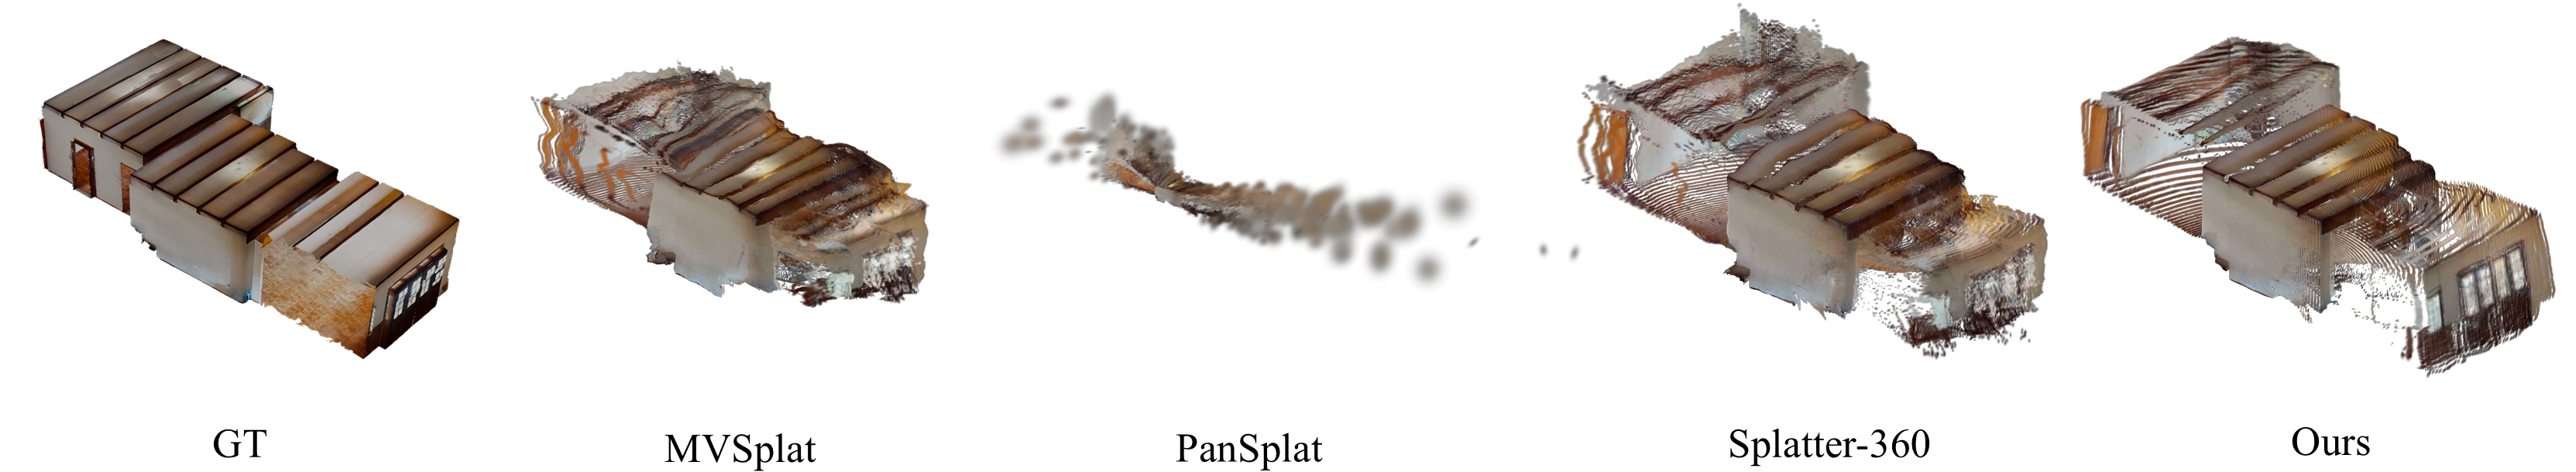
\includegraphics[width=\textwidth]{figures/GS_small.png}
	\caption{Predicted 3D Gaussian spatial distributions of the same scene reconstructed by different methods.}
\label{fig:GS}
\end{center}
\end{figure*}
